\chapter{创新：从个人到公司} % Introduction chapter suppressed from the table of contents

\hypertarget{ux5f15ux8a00}{%
\subsection{引言}\label{ux5f15ux8a00}}

创新，顾名思义，是指创造新的事物或提出与常规不同的见解。

丰田汽车公司精益生产(JIT)的案例展示了丰田通过一线员工的智慧不断改善，最终实现了许多人最初认为不可思议的目标，如“零”缺陷和“零”库存。这使得丰田成为现代汽车生产的标杆。但这些改善都只属于解决问题（Problem Solving），而并非创新（即使团队迭代回顾时针对缺陷排除率分析根因也不能算是创新）。

为什么有些公司和个人能够通过创新取得成功呢？接下来将首先回顾个人创新的要素，然后探索团队创新的方式和成功的关键要素。最后，从这些创新故事中探讨与敏捷开发概念的关系。

创新不仅需要独特的思维和洞察力，更重要的是能否有持久的毅力实现创新。在欧洲文艺复兴初期，一切都要从零开始，创新者必须克服重重困难才能成功。

\hypertarget{ux5e74ux524dux7684ux91cdux5927ux6570ux5b66ux53d1ux660e}{%
\subsection{400年前的重大数学发明}\label{ux5e74ux524dux7684ux91cdux5927ux6570ux5b66ux53d1ux660e}}

如果要你求345乘456等于多少，你可以立即使用电子计算器甚至手机，一秒钟就可以得出准确答案。但在70年代之前（还没有电子计算器），是怎么计算呢？如果用手工计算，很费时间。那时候，许多读理科的学生都使用计算尺（Slide Ruler），通过移动计算尺上的滑动部分来求得答案。

%\href{文件:SlideRulerScreenshot_2023-07-28_182839.jpg}{400px}

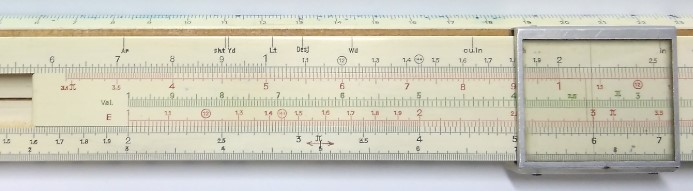
\includegraphics[width=10cm]{SlideRulerScreenshot_2023-12-06_194105.jpg}

对数是计算尺背后的原理。（如果不用计算尺，也可以查对数表得出答案。）

对数是16世纪纳皮尔先生(John Napier 1550 --
1617)用了超过20年时间“发明”的。

\framebox{%
\begin{minipage}[t]{0.97\columnwidth}\raggedright
对数的简单例子：
我们能在草稿纸上计算出 “10,000×100”的结果，同时，我们也可以通过将“10,000”和“100”中的“0”的个数相加，得出答案为“1,000,000”。也就是说,把“10,000”看作是"10”的四次方,把“100”看作是“10”的平方,将四次方和平方的4加2，即可得出答案。纳皮尔注意到了这一数字法则，总结出了对数的概念。

计算``10,000×100''的话，使用乘法会更快，但如果数字位数较大，需要手动计算时，使用加法运算会更加简单。纳皮尔先生按照这思路制作出对数表，简化了计算。

看到这里，也许有读者会想``这不就是指数运算的法则吗？''即是说,按照指数运算的法则``\(a^m \times a^n = a^{m+n}\)''来思考的话，\(10,000 \times 100 = 10^4 \times 10^2 = 10^ {4+2} = 10^6 = 1,000,000\)，如此便可导出答案。然而,在纳皮尔时代并没有指数这种书写方式，指数的概念也不明确。纳皮尔的伟大之处也正在于此，他在没有指数这一概念的情况下发现了对数，并将其归纳为一个体系。
\strut
\end{minipage}}

可以想象在16世纪的欧洲，数学研究还处于早期阶段，发现对数能够将原本复杂耗时的乘法或除法转化为加法或减法进行计算，这是一项非常不容易的成就。为了实现这个方法，他凭借个人努力，花了20年的时间手工计算出相关的对数表。现在我们还可以找到他当时算出的对数表，用现在的计算机验证，8位数运算的头7位还是准确的。

\framebox{%
\begin{minipage}[t]{0.97\columnwidth}\raggedright
纳皮尔先生的对数表： 例如：第一行列出18°30′的正弦值为
0.3173047，对应对数值为 0.111478920。

%\href{文件:微信截图_20230724085408.png}{550px\textbar{}无}
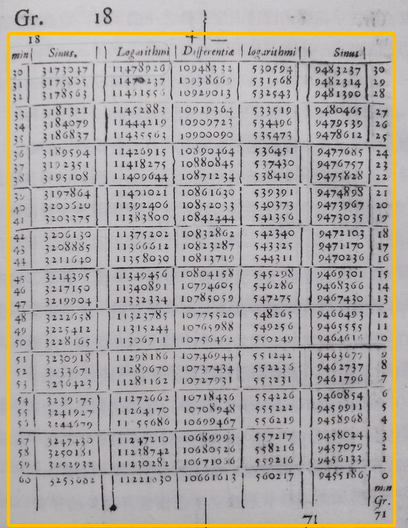
\includegraphics[width=10cm]{微信截图_20230724085408.png}
\strut
\end{minipage}}

当时为什么要计算这些复杂的正弦相乘呢？因为纳皮尔先生还研究球面三角学，可以利用他的纳皮尔公式探究角度与球面弧（距离）之间的关系。16世纪的欧洲国家主要通过航海，发现新大陆进行发展。但海员在大洋中如何确定自己的位置呢？船员在大海中只能依赖天上的星星，利用六分仪估算出船只的经纬度。使用纳皮尔公式，他们就能够估算出地球球面点A和点B之间的弧长。



纳皮尔先生通过研究球面三角学，发现了角度与球面弧（距离）之间的关系公式，如下所示：

\framebox{%
\begin{minipage}[t]{0.97\columnwidth}\raggedright
\(\cos \theta =  \cos \varphi _A\cos \varphi _B\cos\)(
\(\lambda _A\) - \(\lambda _B\) ) +
\(\sin \varphi _A \sin \varphi _B\)
\strut
\end{minipage}}

海员只要知道两点（A和B）的经纬度（角度）便能使用以上纳皮尔公式，估算A和B点之间地球球面弧长。

例子--北京和巴黎距离：

\begin{description}
\tightlist
\item[]
A: 北京中心位于北纬39°54′20″，东经116°25′29″。 转换为纬度 39.905556， 经度
116.424722。

B: 巴黎转换后纬度48.8583 经度 2.29451。
\end{description}

\framebox{%
\begin{minipage}[t]{0.97\columnwidth}\raggedright
\(\cos \theta =  \cos \varphi _A \cos \varphi _B \cos\)(
\(\lambda _A\) - \(\lambda _B\) ) +
\(\sin \varphi _A \sin \varphi _B\)

\begin{description}
\item[]
\begin{description}
\tightlist
\item[]
=\(\cos 39.905556^\circ \times  \cos48.8583^\circ \times \cos\)(\(116.424722^\circ  - 2.29451^\circ\)
) \(+ \sin 39.905556^\circ \times  \sin48.8583 ^\circ\)
\end{description}
\end{description}

\[= 0.767103 \times 0.657923 \times\]（\(-0.40881\)）\(+ 0.64152 \times 0.758084\)

\[= 0.28\]

\[\theta = 1.287\] (rad) AB 距离 = 地球的半径
\(6,378KM \times 1.287 = 8,208KM\) （实际距离是 8,217KM）
\strut
\end{minipage}}
当时没有电子计算机，他发明了对数来解决这类乘除难题（对数不仅仅用于航海，还有助于天文学的计算）。对数帮助我们解决复杂的计算问题长达350年，直到电子计算器出现才退出舞台。


\hypertarget{ux521bux65b0-creativity}{%
\subsection{创新 Creativity}\label{ux521bux65b0-creativity}}

并不是每个人都能像纳皮尔先生那样做出创新和发明，为人类做出巨大贡献。虽然他也是普通人，但又是什么驱动他花费20年的时间和精力来独创对数呢？

\framebox{%
\begin{minipage}[t]{0.97\columnwidth}\raggedright
Robert Fritz 回忆：``60年代，当我在Boston Conservatory
学音乐作曲时，开始思考学的不应仅仅是对位、和音，更要了解音乐大师们的创新过程。''\\
他毕业后继续做音乐创作，有一次参加创新专业人士聚会，这些专业人士中有作家、画家、音乐家和建筑师等，他发现这些人在本专业的创新能力都很强，但都没有想到用他们的创新能力去提升自己的生活。

于是他举办培训课以帮助不同背景的人提升创新能力，让各行各业的人都可以学习什么是创作/创新。几年后，他把创作的重点写成了一本书 (见Reference参考)。Robert Fritz在他的书中，以贝多芬为例，说明创作并非Problem Solving（解决问题），而是要有很高的目标/理想，然后不断地尝试比较，最终达到创作目的。

\strut
\end{minipage}}

\hypertarget{ux521bux9020ux7684ux7cbeux795e-spirit-of-creating}{%
\subsection{原创精神 Spirit of Creating }\label{ux521bux9020ux7684ux7cbeux795e-spirit-of-creating}}

真想不通是什么原因驱动我能够在一个半小时内、在山西省图书馆一口气读完了《且听风吟》(日本著名小说家村上春树先生1973年的处女作品，共144页，共40章)。（快速读完的原因之一是：我没有图书卡，而图书馆会在5点钟准时关门。）

作者描述了自己亲身经历的场景——在酒吧与老朋友喝酒、听电台播放流行歌曲、购买唱片以及邀请女朋友吃牛排等情景。

虽然没有惊天动地的结局，也不是一气呵成的大作风格，相反，里面的场景很散乱。虽然出现了少女裸体、女朋友自杀和作家跳楼等情景，这些都不足以打动我。但总觉得这本书与众不同，很有特色，例如作者本身，以及书中的每一位角色都挺有性格，展现了独立的思维，都是活生生的“真”人。我不仅看到了他们的表面，也感受到了他们内心深处的世界。

创作并非被他人驱使，而是源自内心对创作的渴望，渴望创作出世界上最优秀的作品。只有认为自己的创作具有重要价值，才会尽全力努力创作。最终，希望自己的作品拥有独特的生命力，并受到他人的赞赏。

除了《且听风吟》，我还读过《挪威的森林》，也是采用第一人称叙述的手法，以作者渡边君的视角逐步展开各角色：例如他好朋友本月的女友直子，大学同学绿子，在疗养院照顾直子的玲子等。直子的优美、优雅、娴静，绿子的活泼烂漫，都是通过渡边的亲身经历逐步细化而来，就像使用显微镜观察一个细胞：起初由于焦距还没有对好，一片模糊，但随着焦距的调整，可以一步步看清细胞的每一个细节。每个故事的发展也时不时地出人意料，就像一部优秀的话剧，观众永远无法预料下一个桥段……这种情节的安排吸引着读者继续追读，让他们不愿停下来。（因为延续了《且听风吟》的写作风格，有些评论就认为《挪威的森林》运用了大量无意义的描写，这些描写空洞、无新意，仿佛只是为了拼凑字数与拖缓节奏而存在） 

《海边的卡夫卡》于2002年出版。在这本书里，村上先生设立了卡夫卡和中田两条线，奇数章以卡夫卡的故事为主线，偶数章则以中田的故事为主线，两条主线齐头并进。起初两条线没有直接的交叉点，但后来它们产生了交集。像我这样的非文科读者可能会觉得两条独立的情节主线会很奇怪，但当它们开始产生交集时，便会感到耳目一新——从没有过类似的小说。 

文艺创作，无论文学或音乐，不同于数学、科学，给作者很多原创的空间，贝多芬的创新推动了西方音乐从古典时期向浪漫时期的过渡。 

\framebox{%
\begin{minipage}[t]{0.97\columnwidth}\raggedright

贝多芬 (1770 – 1827)的音乐创新可以说是前无古人后无来者，深深影响着后面两个世纪的作曲家。

我们都熟悉他的《命运交响曲》，其实从1795年到1827年他去世前，他出版的每一首作品，不论是交响曲、室内乐还是歌剧，都堪称经典。他是完美主义者，例如《田园交响曲》的创作时间不少于3年，从他手稿得知，首乐章某主题他修改了不下12次，所以与巴赫、莫扎特、舒伯特比较，他的“生产率”不算高，平均每年出版5~6个作品。
他出版《命运交响曲》、《田园交响曲》时(1808)，已经出版音乐作品13年，包括23首钢琴奏鸣曲，9首弦乐四重奏。

贝多芬的早期作品风格与海顿和莫扎特还很相似，但到了中期，如《命运交响曲》和《田园交响曲》，就已经远远超越了他的前辈和同辈们，并启发音乐家们从古典主义逐渐发展出浪漫主义的新风格。

例如，在《第九交响曲》最后的第四乐章中引入了四声部合唱，这在传统的交响曲中也是前所未有的（传统交响曲通常只由乐队演奏）。

贝多芬晚期的作品，如钢琴曲和弦乐四重奏等，又展现出了与中前期不同的另一种风格。例如，他的作品Op133弦乐四重奏Große Fuge，由于其思想深邃远超当时的水平，并未被当时的音乐家所接受，他们认为这部作品有问题，有的甚至批评他太老了，不仅聋了还疯了。但贝多芬仍然故我，表示：“这首曲子就是为未来而写的！”

\strut
\end{minipage}}


%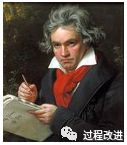
\includegraphics[width=10cm]{Bdf.png}

很多人都听过贝多芬的钢琴奏鸣曲，例如《悲怆》、《月光》奏鸣曲等。我也觉得他的钢琴曲与莫扎特和他老师海顿不同，别具一格。


贝多芬对音乐创作的远景目标——希望创造前所未有的作品（他觉得当代的作品，甚至包括海顿和莫扎特的作品，离这远景还差很远）。由这崇高的目标驱动，加上他自身的音乐演奏和作曲能力，贝多芬不断突破，甚至连耳聋也阻挡不了他的创作力（他从25岁开始听力减退，到45岁已经完全失聪），将音乐创作推向了新的高度，对后来的作曲家产生了深远的影响。
贝多芬追求完美，他有极大的魄力，通过持续不断地创新和完善，这才取得了超越常人的成就。


Fritz 发现大师们都拥有以下共同的特点：把握自己的命运，和主动追求个人目标。许多人很有才华，但为什么他们中的大多数却不能成为大师？他用下图解释。除了要对未来有远景目标外，了解现状同样重要。如果不觉得有差距（张力），就没有改进的驱动力。有些人有理想，但缺乏计划与行动，便只是梦想。 

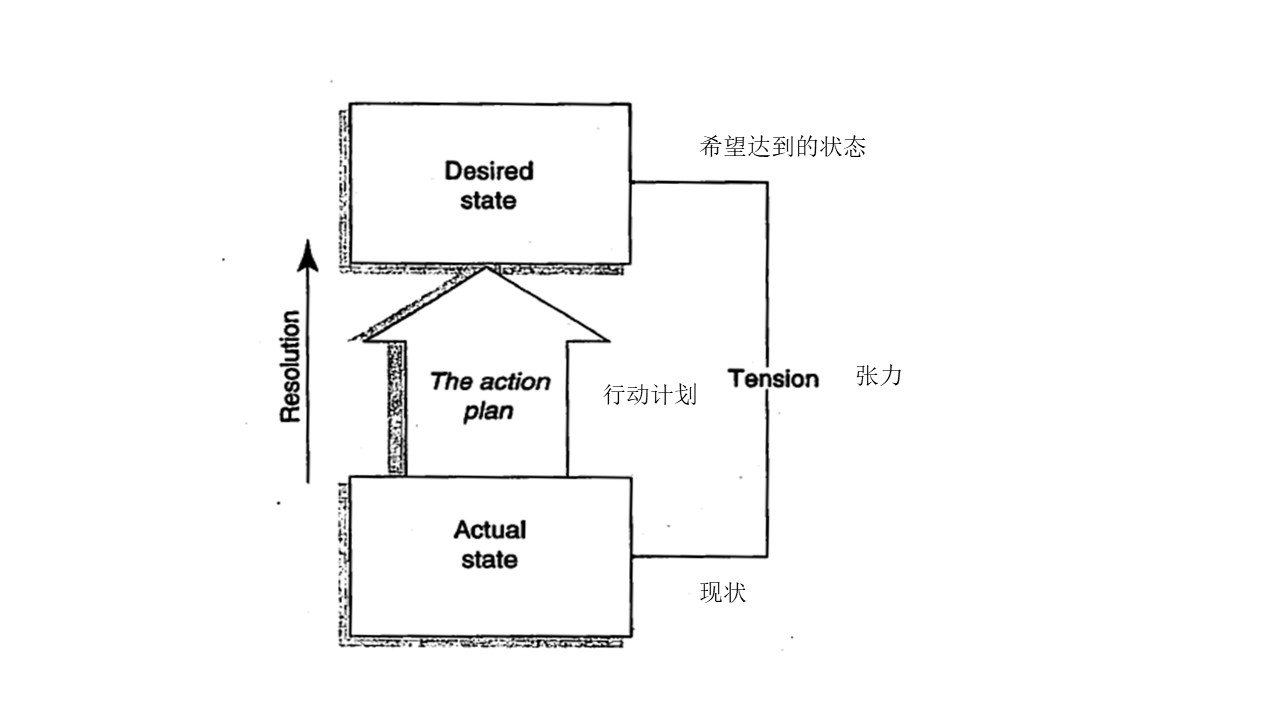
\includegraphics[width=10cm]{Liuct.png}

这个创新驱动模型不仅仅适用于音乐创作，也适用于数学。例如，纳皮尔先生为了解决正弦相乘的困难，发现可以转换成对数进行计算，把乘法简化为加法(VISION)，为了实用，又花毕生精力计算出了对数表，也是从张力转化为行动(ACTION)并创新的例子。 

从贝多芬和村上春树的故事中，我们了解到创新首先是由不满足于现状驱动、并由此长期不断完善的结果。如村上先生说：并非受人之托才写小说，而是因为”我想写小说"这种强烈愿望，深刻感受到这种内在动力，才不辞劳苦地努力写小说。 



\hypertarget{ux516cux53f8ux5982ux4f55ux521bux65b0}{%
\subsection{公司如何创新}\label{ux516cux53f8ux5982ux4f55ux521bux65b0}}

\framebox{%
\begin{minipage}[t]{0.97\columnwidth}\raggedright
您身边的人群中可能有超过50%的人都在使用这家公司的产品，涵盖各个年龄段。该公司的产品功能广泛，包括音乐播放、电话、电脑/平板、在线视频观看以及日常工作。您能猜到这家公司的名字吗？

\strut
\end{minipage}}

苹果公司 (Apple)

我和全世界千千万万人一样每天都在使用苹果产品：iPhone、iPAD平板电脑和iTune网上搜索音乐歌曲，要了解苹果的成就，就不能不谈乔布斯 (Steve Jobs)了。他的一生充满传奇，很多故事可通过阅读《Steve Jobs》一书进行了解。让我们先回顾苹果如何成为大众音乐市场巨人的故事。

\begin{description}
\item[]
\begin{description}
\tightlist
\item[]
= = =
\end{description}
\end{description}

\hypertarget{ux97f3ux4e50ux64adux653eux5668}{%
\subsection{音乐播放器}\label{ux97f3ux4e50ux64adux653eux5668}}

自80年代末MP3格式问世以来，将歌曲数字化开始流行，市场上也出现了一些可以随身携带听音乐的小型设备。然而，由于技术限制， 这些设备都存在不少问题。他们比较了当时市场上常见的播放器，发现或多或少存在各种问题，例如容量有限、难以按照个人喜好进行歌曲的排序等，如果想要从CD上下载歌曲到电脑，然后按照自己的喜 好顺序在播放器上播放，过程相当复杂。乔布斯本人很喜欢音乐，他看准了这个市场，并希望将苹果电脑定位为个人电子设备（包括音乐播放器）的综合中心 (Hub)。首先要解决的是音乐播放器的便携性和存储容量。当时，小型显示器、锂电池和小型硬盘都尚未普及。几个月后，他 们找到了合适的解决方案:东芝刚刚研发出一款直径只有一英寸的超小型5G硬盘，形状像个大银币。但如果将这些功能都集成到播放器中去实现，因为播放器的屏幕尺寸太小了，实现起来非常困难。他一直非常关注产品的易用性,当乔布斯看完内部软件研发工程师首次展示正在开发中的刻录软件后，他站到白板前画了一个框，说：“你们设计的软件就应该只需把歌曲拉到那个框里面，然后点击一个按钮就可以刻录。”当时软件工程师被吓呆了，觉得很难做到。这反映工程师往往不会从用户的角度来看问题，乔布斯后来要求播放器软件都必须给不懂技术的人使用，让她在3个步骤内，不需要查看说明书就能完成任务，这成为他的测试标准，如果做不到，他就不会接受这软件。播放器的设计也有创新，比如通过转动面板上的轮子来选择歌曲，用户只需转动轮子就能方便地跳到要听的歌曲，这样的设计极为便捷。iPod的产品设计也体现了苹果公司一贯的设计理念——简洁。产品采用白色设计，包括耳机在内都是白色（当时，大部分耳机还是黑色的），甚至连充电器也是白色的。设计师Jony Ive 解释：“白色能够赋予产品高贵感，使其与其他廉价的播放器有明显区别，用户会觉得这样的设计有艺术感。”


%\href{文件:R-C_(2)_副本.jpg}{350px}

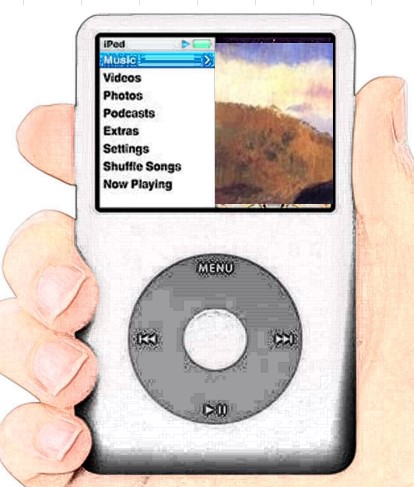
\includegraphics[width=10cm]{!ipodcutoutScreenshot_2023-12-06_201652.jpg}

乔布斯也非常注重产品包装，iPod的包装让你觉得：``在拆包装时，觉得有一件很贵重的东西在里面''。

%\href{文件:IpodPackageScreenshot_2023-07-23_201312_labi.jpg}{400px\textbar{}无}

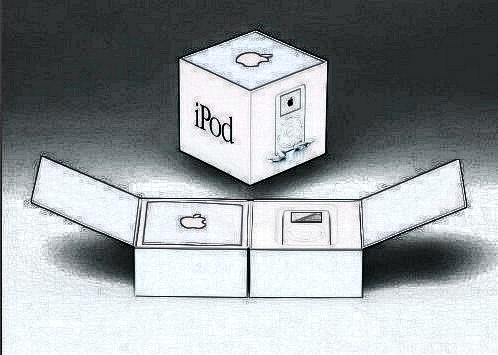
\includegraphics[width=10cm]{IpodPackageScreenshot_2023-07-23_201312_labi.jpg}

虽然定价不低：399美元，很多人觉得定价过高，但是iPod在2002年正式推出市场后一直热卖。

\begin{description}
\tightlist
\item[]
= = = =
\end{description}

从2001年到2014年苹果大概卖出了4亿件iPod，2015年后还继续卖出50,000,000件。iPod播放器也成为了苹果的主要收入来源。2006 年，也就是苹果推出iPhone的前一年，iPod的销售收入占了公司总收入的40%。下图展示了从2002到2013年，iPod的销售数量变化和收入占比变化：

%\href{文件:IPodRiseFallScreenshot_2023-07-22_164335.jpg}{300px}

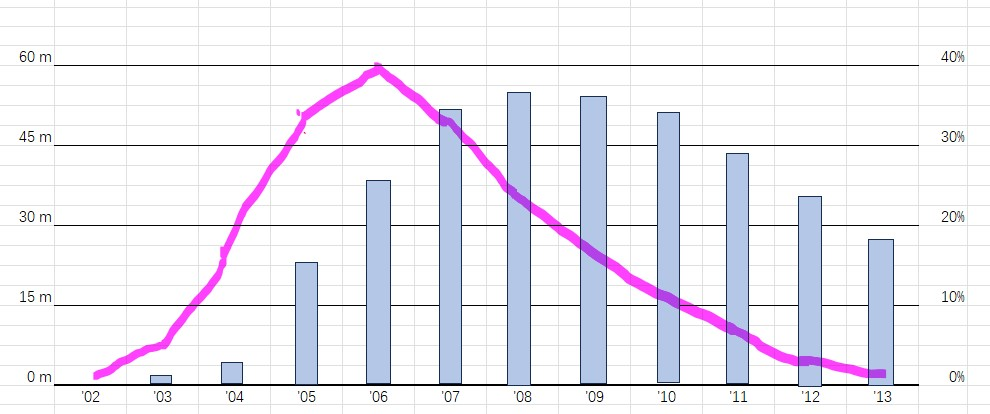
\includegraphics[width=10cm]{AppleRiseFallDrawScreenshot_2023-12-06_211749.jpg}

\hypertarget{itunes-ux7f51ux4e0aux5546ux5e97}{%
\subsection{iTunes 网上商店}\label{itunes-ux7f51ux4e0aux5546ux5e97}}

苹果的iPod加上Mac电脑的iTune应用软件很成功，但这只解决了从网上下载音乐并在便携播放器听歌的技术问题，还有更严重的问题需要解决——盗版，2000年开始，越来越多网站提供免费音乐下载，这不单影响了唱片销售（2002年销售额下降了9%），也侵犯了音乐创作者的知识产权。各大唱片公司都急于解决这一问题，但大多数公司缺乏所需的技术能力。乔布斯也十分重视这些创作者的利益，他预见到如果没有知识产权的保护，就不会有人再有动力录制高质量的音乐作品（就像没有知识产权保护，就没有软件和电脑公司愿意投资进行创新）。

因此，他基于iPod和iTunes音乐播放能与电脑结合的特点，向各大唱片公司展示了在线平台如何运作、如何防止盗版。由于唱片公司缺乏相关的技术，很快就有4家唱片公司表示有兴趣，愿意合作：利用iPod、iTunes等技术，筹建统一在线平台服务，使消费者可以在网上购买并下载音乐。

从2002年开始，乔布斯一直忙于周旋各类问题：除了技术方面格式问题要解决（例如各有自己的格式，需要统一），也有些唱片公司想保护自身利益（例如索尼，自身实力雄厚，有意建立自己的音乐平台）。

最终在2003年4月，iTunes store 正式推出市场，用户可以在网上用关键字搜索任何一家唱片公司的唱片或歌曲，也可以搜索相关的唱片。乔布斯的业务模式很简单，他从以前的经验知道首先要通过低价吸引大量用户使用，如果收费太高，只是小部分人使用，就流行不起来，也没有动力吸引新唱片公司加入，恶性循环。他的策略很成功。

2003年苹果刚开始发布iTunes 网上商店时有200,000歌曲可以下载购买。他本来预计可能需要6个月的时间才能售出100万首歌曲。但实际上推出6天就已经卖了100万，到2003年12月，已经累计卖出2500万首歌曲。

2004年7月份共卖出一亿首歌曲（2003年底的4倍）；2005年11月（两年半后）苹果成为全美国十大音乐零售商之一，其他都是传统零售商，例如第一是Walmart。

随着网上买歌商业模式越来越普遍，传统零售商越来越困难，到了2010年2月，苹果成为美国最大的音乐零售商。

因为网络技术发达，现在不再是当年的网上下载，但很多人还是喜欢只须要每个月交几十块钱就可以随时随意在网上搜索并听到自己心爱的歌曲，这商业模式也保护了艺术家、唱片公司的利益。


从以上乔布斯关于音乐的故事，我们可以看到与400年前相比，创新的速度发生了巨大的变化。在过去，像纳皮尔那样仅凭一个人独立完成创新可能需要20年的时间。到了2000年，一切都变得非常迅速，乔布斯的团队只用3个月就推出了iPod播放器，并在两年内创建了iTunes网上音乐平台，帮助苹果公司为个人客户提供数字中心（Digital Hub）平台服务。客户可以使用电脑选择喜爱的歌曲在iPod 播放，也可以下载最新的歌曲，非常方便。这些就是我们2000年代看到的创新，这些创新不可能靠一个人独自完成，而是要团队合作。

公司创新与几百年前那些大师的创新最大的区别：需要整个公司所有人的协作，并确保他们的目标一致。这意味着整个组织的各个部门都必须协调合作，同时又要细分目标，以便不同的人负责执行不同的任务。


纳皮尔先生花了20年时间写了3本数学书，总页数不到200页（其中一本还是在他去世后出版的），贝多芬的产量也不算高，一年只出版几首作品。这些大师都是靠个人的努力完成整个创作过程。但是现代市场变化越来越快，要成功，公司必须快人一步，但因依赖团队合作（各有专长），也需要协调大家的工作，确保各个层次的目标与公司总目标一致。
下面介绍一个简单的系统让企业管理整个公司的提升：

   1. 识别公司的总目标。\\

        例如在下一年，要一年内生产7个新的产品系统。\\

   2.描述公司的现状。\\

        例如现状是：平均一年只能产出3个新产品，有2个开发团队。但开发人员的能力有限，质量也不好，导致用了不少精力，去维护已经完成的产品，没有时间来开发新的，招新人也不容易，比较难找得合适的，也没有时间培养新人，扩大工作。

    3.形成具体行动计划。\\

        例如简洁、精简的开发流程，增加1个开发团队，加强代码评审和编码能力，来减少缺陷导致的返工，要跟市场部密切合作，确保新产品满足客户的要求，给客户带来价值。
        但真正公司的从上而下总计划会更具体。\\

    4.当我们定好明确的最终结果，也了解真正的现状，有一些行动计划，下一步是具体到每活动的完成日期和负责人。\\

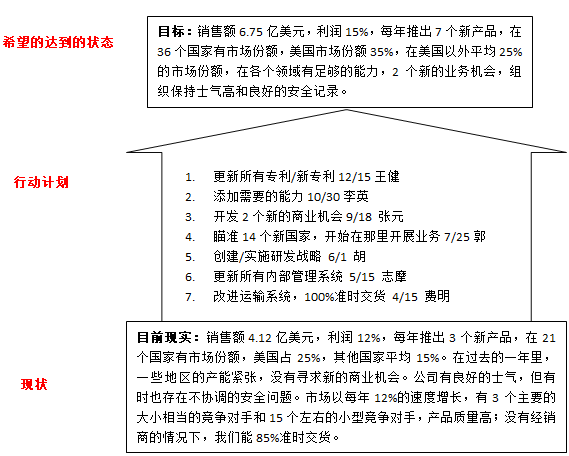
\includegraphics[width=10cm]{385页替换图片.png}

同意可以用以上模式帮助公司创新吗？ 先回顾村上先生的40年创作经历：

\framebox{%
\begin{minipage}[t]{0.97\columnwidth}\raggedright
村上春树先生《 我的职业是小说家 》

    （2017年出版，他当时68岁，从73年出版《且听风吟》开始,他已经不停写书超过40年）

写长篇小说是我的“主业”，我规定自己每天写10页稿纸，每页400字，形成规律。1987年出版的《挪威的森林》，全部的书稿是我在欧洲旅行期间写的，因为不熟悉当地的环境，每天都要费一番功夫才找到一个咖啡厅写稿，但我依然保持每天10页的写作量。
然后我进行了多轮修改。修改十分重要，例如我在欧洲创作《舞!舞!舞!》(1988年出版)，开始使用富士通便携式计算机写稿)时，临发稿时才突然发现有一篇我觉得写得挺好的章节找不到了，只好按照原来的思路重写。书出版后，又突然在电脑里发现了那篇章节，原来是放在一个很少用的文件夹里。但我发现出版的版本远远比旧版好，所以不断修改是非常必要的。
写小说需要灵感，因此必须阅读大量作品，不仅仅只是名家的作品。我的小说主要描述各种人物，所以我会细心观察他们的特征，并将其展现在小说中。就像风景油画家必须仔细观察周围景色的颜色和光线一样。1979年，我的第一本小说《且听风吟》得了新人奖时，我的高中老同学来到我开的小店说：“你那种玩儿都行的话，我也能写出来。”他说完就走了。真奇怪，虽然当时我很气愤，但也自己想：“说不定真像那个家伙说的，那种水平的玩意儿，只怕谁都能写出来。”我仅仅是运用简单的文字，把浮上脑际的东西记录下来。艰深的词语、考究的表达、流利的文体一样也没用到，说来几乎无异于“空洞无物”。
我从那“空洞无物”、简单的文体开始，写出一部部作品，注入血肉，将规模更大更加复杂的故事塞进其中。从得新人奖的第一部小说起，到现在已经过了40年，我一直都在从事这项工作。到事后回顾才发现一直只是一步一步逐渐完善，并不是从一开始就计划周全、按部就班完成的。 

\strut
\end{minipage}}

个人的创新已经不可以预先规划，公司面对的外部与内部变数更多，更无法预先策划。 我们看看乔布斯另外两个公司的创新故事。


\hypertarget{ux516cux53f8ux5982ux4f55ux521bux65b0-1}{%
\subsection{万事起头难}\label{ux516cux53f8ux5982ux4f55ux521bux65b0-1}}

985年9月，乔布斯被迫离开苹果公司后，自己投资700万美元，创立了一家专门针对高校工作站市场的新公司，名为NeXT。乔布斯开始时对公司的期望特别高，当时他看到这市场主要被太阳（SUN） 和（DEC） 公司占有，但这些工作站产品都是以输入命令为主，与Macintosh用鼠标操作不同，所以易用性不高，所以他希望创造前所未有的新平台，让那些高校的学者与研究人员可以简单地使用电脑模拟各种场景来做研究。

但是要达到这么高的理想，要做的工作就非常多。比如第一次公司开创90天后就开始有一次度假村的头脑风暴会议，希望可以在两年后推出产品，以赶上学校放暑假购买电脑的时机。三个月后再次讨论时，大家都意识到这个目标太高，难以实现。但乔布斯没有放弃，他一直用自己的魅力说我们可以按大家的专长达到这个目标。
1986年过去，1987年又过去了，但新产品研发仍然没有显著进展。直到1988年，公司才进行了第一次长达3个小时的产品演示，但产品仍然处于初级阶段，没有彩色显示，并且速度较慢。尽管签下了曾为苹果推销Mac的全国电脑零售商，但一年仅售出360台，与预期相差甚远。（在1984年，同一家全国零售商却为苹果售出了40万台Mac；而NeXT工厂的生产线设计标准是每月生产1000台产品。）

1990年，到公司的第二次产品发布时，新产品开始用了彩色显示，速度也得到了提升。然而，尽管有所改进，该产品仍然被认为只是初级产品，尚未完全成熟。
由于销售情况不理想，乔布斯再次投入了500万美元的资金，但很快就用光了。幸运的是，有一位外部投资者——德州企业家Ross Perot先生，他对乔布斯非常信任（他觉得以前没有来得及投资苹果，一直耿耿于怀），因此投资了2000万美元进入NeXT。
1993年，公司开始裁员。600人的公司，起初只裁减了几十人，随后又裁掉了200多人，接近公司总人数的一半，随后又有200多人被裁，最终公司将整个硬件部门出售给了日本佳能公司，只保留了操作系统部分NextStep。因为苹果公司看中了该操作系统，NeXT公司于1996年以4300万美元的价格被苹果收购，乔布斯也得以重返苹果公司（最初以顾问身份）。又经过了15年的努力，乔布斯带领苹果公司再度走向辉煌。 

\hypertarget{ux516cux53f8ux5982ux4f55ux521bux65b0-1}{%
\subsection{从濒临破产变为回报最好的投资}\label{ux516cux53f8ux5982ux4f55ux521bux65b0-1}}

乔布斯在1986年用一千万美元投资Pixar。当时，Pixar只是LucasFilm旗下的一个由30多人组成的电脑部，由《星球大战》导演George Lucas创立，主要用于电影动漫效果的制作。乔布斯对美术领域一直很感兴趣，他通过Alan Kay的介绍去参观了Pixar，被公司的产品深深吸引，认为其技术领先并远超同行。乔布斯最初只是一名投资者，并没有过多干预公司的软硬件产品开发，但乔布斯雄心勃勃，觉得公司开发的产品有特长，也希望能像苹果的Mac一样，大量供给动漫专业人员，进行3D设计。尽管产品的功能强大，但使用起来仍需要复杂的命令操作，不太适合一般的动漫从业者（Adobe推出的软件，虽然功能不如Pixar强大，但更易于上手）。因此，乔布斯投入了更多研发资源，改善产品的易用性。为了推广Pixar产品，他开设了很多零售商店。
虽然乔布斯对Pixar公司的投资不断增加，然而产品的销售情况一直未见起色，公司陷入了资金短缺的境地。到了1988年，他被迫采取了紧缩开支和裁员的措施。直到1991年，与迪士尼合作制作Toy Story《玩具总动员》，Pixar才得以起死回生。乔布斯在这之前已经投入了高达5千万美元的资金，相当于他从苹果公司股票出售所得收入的一半。因为与迪士尼的成功合作，Pixar公司得以在1995年（与Toy Story首次公演同年）成功上市，获得了15亿美元投资。随后，Pixar与迪士尼继续合作，推出了5部动漫电影，都非常卖座。2006年，迪士尼为了防止Pixar与其他公司合作，以74亿美元的价格收购了Pixar，也使乔布斯成为迪士尼的最大独立股东。（关于Pixar Toy Story制作故事，请看附件） 


\framebox{%
\begin{minipage}[t]{0.97\columnwidth}\raggedright
后来的事实证明，乔布斯认为一般动漫从业者会喜欢使用Pixar的3D建模软件是错误的，这只是他的一厢情愿。但他的另一个希望：如何结合电脑数字技术和艺术做创新，确保梦想成真，Pixar与迪士尼合作制作新一代动漫片，从1995年的Toy Story开始，把动画片技术提升一个高度。

\strut
\end{minipage}}

从以上两个案例可以看出，任何企业的创新往往会面临难以预料的挑战。因为市场的不确定性，超过90%的创新产品可能最终以失败告终，因此可能并不适用于传统的企业策划方式。这也印证了马云先生的名言：“今天很残酷，明天更残酷，后天会很美好，但绝大多数人都死在明天晚上”。


\hypertarget{ux516cux53f8ux5982ux4f55ux521bux65b0-1}{%
\subsection{公司创新成功要素}\label{ux516cux53f8ux5982ux4f55ux521bux65b0-1}}

回顾iTunes电子商店和之前iPod成功的故事，以及乔布斯与NeXT和Pixar的故事，可以总结出以下成功要素和注意事项： 

\hypertarget{ux7075ux6d3bux654fux6377}{%
\subsubsection{灵活、敏捷}\label{ux7075ux6d3bux654fux6377}}

从达尔文物种进化历史可以看到物种可持续的原则：

\begin{itemize}
\tightlist
\item
  最强壮/巨大的物种也会灭绝（如猛犸象）
\item
  只有最能快速适应环境变化的物种才能长期传承下去
\end{itemize}

从60年代开始，商业环境快速变化，也只有能快速适应环境的公司，不断求变，才能持久，成为百年老店。

从乔布斯的NeXT和Pixar故事可以看出，创建新产品或服务涉及诸多不确定因素，失败的可能性很大。因此必须随时调整策略以适应变化。如果发现最初的想法或计划没有产生预期的效果，就应立即做出改变。

这个原则适用于许多科技公司，比如谷歌，它也有很多失败的项目。谷歌的宗旨是“Fail Fast”，意思是如果一个项目在半年到九个月内未能达到一定的客户量，就会立即终止该项目。许多科技公司通常在年底才会全面评估某项业务是否可持续，但为时已晚。

这也是敏捷开发的原则之一：不将精力集中在长远的规划上。由于需求经常变化，敏捷开发将项目分解成小迭代，每个迭代都是一个冲刺，以有限的资源尽力做好每个迭代：这不仅提升了效率，而且产品质量也会更好。

\hypertarget{ux4e13ux6ce8focus}{%
\subsubsection{专注(Focus)}\label{ux4e13ux6ce8focus}}

资源有限，公司应该专注于自身能够做好的事情，而将那些可以外包的任务尽量外包。举例来说，对于生产方面，苹果公司专注于发挥自身的专长——产品设计。（请不要误解苹果公司对生产的态度，它的产品生产都是按照JIT原则组织的，只是不直接雇佣生产工人。）


乔布斯回到苹果后，吸取了过去十年在NeXT和Pixar的经验教训。当时苹果公司内部存在着一百多个研发项目，乔布斯深知资源的有限性，因此开始对这些项目进行整合。他只保留了在市场上表现最优秀的项目，解散了那些不必要的研发团队，只保留与公司发展愿景相关的研发项目。

乔布斯2010年被访问时说：“我们选技术，只挑选有发展潜力的技术，如果什么都支持、都研究就会耗费宝贵资源。”

\hypertarget{aux7ea7ux56e2ux961fux6210ux5458}{%
\subsubsection{A级团队成员}\label{aux7ea7ux56e2ux961fux6210ux5458}}

Pixar公司虽然小，但每位都是行业精英。

\framebox{%
\begin{minipage}[t]{0.97\columnwidth}\raggedright
我在美国的堂弟从小就对动画人物情有独钟，家中也都是星际旅行、星球大战等的模型。他来香港旅游时还特意光顾那些专门销售他喜欢的卡通人物模型的小店。他（读建筑专业）毕业后专攻动画片和主题乐园设计。

他和其他3位设计师是公司外聘参加超人总动员》制作设计的原始核心团队。其他3位都是行业中的有名高手，例如，Blackman
曾设计蝙蝠侠系列，Delgado 设计星际旅行(Star Trek)等。

他说``Pixar公司在动画片行业非常出名。
核心制作团队,包括艺术总监和生产设计师等都是当时行业的顶尖高手，
他们除了能力超强，对艺术创作的品味与兴趣跟我也很相似，能有这机会与他们共事合作
真是非常幸运，像中了彩票一样。开始时，我们四位设计主要成员定期要跟导演Brad
Bird 开会，评审设计。``
超人总动员》非常卖座，美国本土票房收入已经超过2亿美元，也得了奥斯卡奖。

Pixar公司这些动画片，能有这么好的票房，并得奖，不是没有原因的，因为公司有名气，可以吸引到当时最优秀的艺术家参加，有了这些人，我们才可以看到像《超人总动员》这档次的高端制作。
\strut
\end{minipage}}

因此，当A级成员遇上能力相当的团队伙伴时，能够激发更大的创造力，产生1+1>2的效果。

苹果公司于1984年推出的Macintosh，产品在技术能力和设计方面（如视窗、鼠标等），远远领先于之前IBM推出的IBM PC。该产品的开发团队成员也都能力超群：其中， Burrell Smith负责硬件线路板设计，Andy Hertzfeld等人负责Mac GUI操作系统的设计，Bill Atkinson负责Graphics应用软件QuickDraw和HyperCard的设计，Joanna Hoffman负责市场推广，Bruce Horn负责Resource Manager 应用软件的设计等。然而产品推出后，因销售情况并不理想，管理层也发生了变动，导致团队成员陆续离开。

乔布斯从Pixar的经验，深明高端球员(A
Players)只愿意与高端球员搭档的道理。但为了吸引和留住这些精英，公司必须给有吸引力的报酬。

例如，乔回苹果不久就特别要求董事会修订员工股权安排（因当时苹果股价已经很低，之前的员工股权安排已经没有意义。）

\hypertarget{ux6781ux9ad8ux76eeux6807ux8981ux505aux5927ux505aux5f3a}{%
\subsubsection{极高目标，要做大做强}\label{ux6781ux9ad8ux76eeux6807ux8981ux505aux5927ux505aux5f3a}}

\framebox{%
\begin{minipage}[t]{0.97\columnwidth}\raggedright
在杭州某商务酒店看到十几条浙商名言，写在墙上，其中一条如下：

%\href{文件:mingyant.png}{600px}
\includegraphics[width=10cm]{mingyant.png}
\strut
\end{minipage}}

乔布斯创立NeXT时是世界第一的工作站供应商，所以生产线是按每月能生产一千台设计！他重返苹果后，一直秉持着以创造世界第一的产品为目标，这在后来被证明是成功的，例如iPod/iTunes(2001)、iPhone(2007)、iPad(2010)等。这种思路使得苹果公司成为了美国市值最大的科技公司。


正如丰田的大野耐一所说：“容易达成的目标并不是好目标”，他给丰田员工设定的质量目标是零缺陷。

\hypertarget{ux6709ux975eux5e38ux9ad8ux7684ux8981ux6c42ux7528ux5fc3ux505a}{%
\subsubsection{有非常高的要求，用心做}\label{ux6709ux975eux5e38ux9ad8ux7684ux8981ux6c42ux7528ux5fc3ux505a}}

每位团队成员都应该追求卓越，不仅仅是完成任务，而是要创造出优秀的、世界一流的产品。只有这种抱负才能激发每个人付出最大的努力，把事情做好。乔布斯本人就是一个典型的例子，他判断有价值事就会全力以赴去做到最好。举例来说，在推出iTunes电子商店之前，他就不断地邀请各种音乐家、歌手和音乐制作人参与其中。他每次都会想尽办法去介绍他的好东西，有一次小号手W. Marsalis到家拜访，乔布斯就问他：“你喜欢谁的作品？”

Marsalis
说：``贝多芬''，他就一起展示如何在商店里面可以容易搜索到贝多芬的作品，Marsalis后面回顾说：“其实我一直都对电脑不太感兴趣，但乔布斯他一直全心全意，全程用了两个小时很细心地给我介绍。过了一会，我的注意力不是放在他的产品或者电脑上，而是他本人，我深深地被他的激情和专注打动了。”

例如苹果的首席设计师 Jony Ive
用简洁设计思路，让消费者觉得苹果产品有艺术感，非一般电脑：

%\href{文件:Power_Mac_Screenshot_2023-07-05_131914_副本.jpg}{300px}

%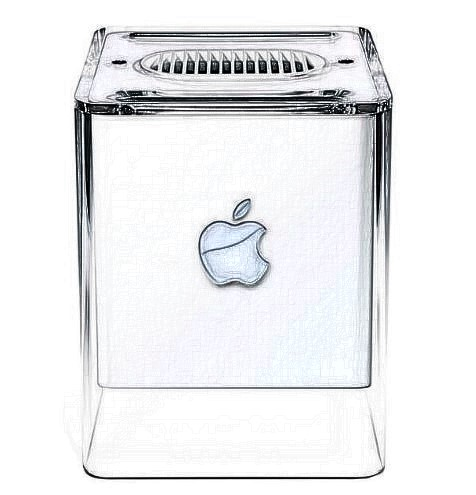
\includegraphics[width=10cm]{Power_Mac_Screenshot_2023-07-05_131914_副本.jpg}

%\href{文件:R-C_副本.jpg}{300px}

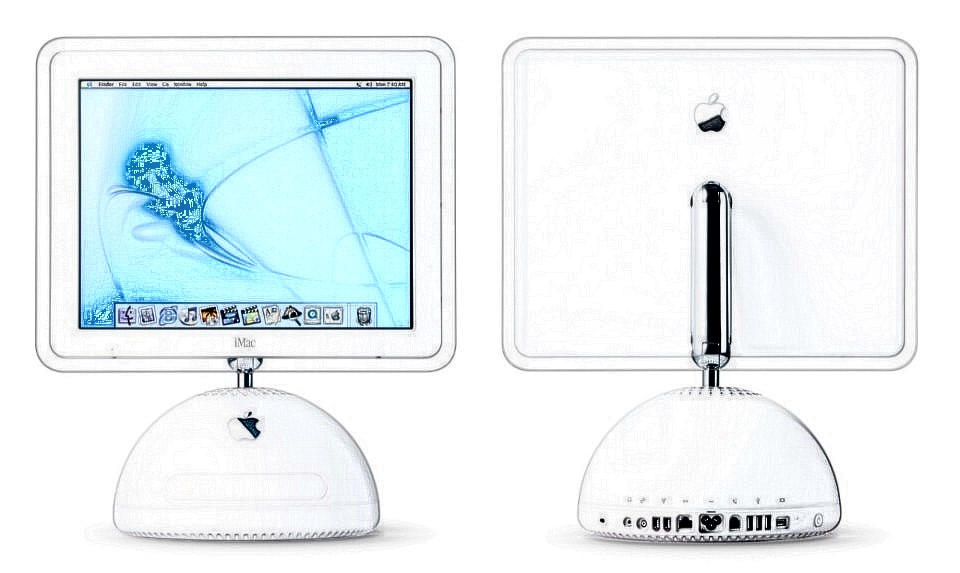
\includegraphics[width=10cm]{R-C_副本.jpg}

Ive的父亲是位优秀工匠，从父亲那他学到要做一流工匠必须对质量有极高要求。

\hypertarget{ux9886ux5bfcux51b3ux7b56ux5febux901fux884cux52a8}{%
\subsubsection{领导决策、快速行动}\label{ux9886ux5bfcux51b3ux7b56ux5febux901fux884cux52a8}}

索尼一直以其在电子产品领域的创新而闻名，例如Walkman，同时也拥有唱片公司；创建网上音乐平台的主要条件它都具备了，但为何索尼做不到，苹果却成功了呢？其中最大的原因在于索尼是一家庞大的企业，由各个事业部门组成，每个事业部门都要追求自身的盈利。正是这个原因，当需要各团队之间进行紧密协作时，许多精力就被耗费在部门之间的协调上，最终以失败告终。相反苹果公司不是这样的，它只关注整个公司的总体利益，而且乔布斯对产品有着非常高的要求。例如，在设计iPod的时候，工程部和软件开发部门完成了30个原型初稿后，乔布斯参与讨论后立即确定了设计方案，随后就立即着手实施了。（有些在其他大公司，比如飞利浦，工作过的员工会觉得很奇怪，因为像西门子、飞利浦那种传统大公司绝对不会在一个会议里做这么重大的设计决策。）


\hypertarget{ux7ed3ux675fux8bed}{%
\subsection{结束语}\label{ux7ed3ux675fux8bed}}

苹果的案例可以被视为将敏捷开发升级至企业级的最佳实践案例，从前面的故事中可以看出，整个公司都在按照精益的思路不断改善。

团队合作至关重要，而团队成员的能力要求也很高，这样才能在最短的时间内做到最好。强调岗位之间的相互合作，不是将工作分得很细，比如你负责测试，我负责开发，各自只需要做好自己的工作，而是要求团队成员相互协作，最终确保整个项目或产品的成功。不应计较是否在自己的工作范围之内，应该确保成员之间相互有效沟通，即使在需求或开发方面是最优秀的，但并不代表产品能做到最优。有些开发团队会抱怨说：“其实我们的开发工作做得挺不错的，但是由于需求混乱，我们无法做到最好。”

但是因为公司架构原因，部门之间各有自己的指标，导致各功能之间不能相互合作做好。

从乔布斯的故事中了解到，高层对产品质量有极高的要求这一点至关重要，敏捷开发也同样。如果敏捷团队不注重产品质量，只关注按时交付，最后只能生产出一些不达标的次等产品。但反过来，当团队具备足够的能力，并且大家都有抱负、有追求，敏捷开发可以帮助团队快速响应不断变化的需求，就像苹果和乔布斯一样，成为世界第一。

1983 ~ 
84年，乔布斯（28岁）在苹果公司带领Mackintosh开发团队时，就不会向预计交付期限低头。如果他觉得产品未达到质量要求，他宁愿延后。他甚至鼓励团员要精益求精。（千万不要以为你在他管理的团队可以偷懒）

有人问我：“听说过SAFe这个框架吗？我们想用它在公司级别推行敏捷，你觉得怎么样？

我：框架就只是框架，如果没有刚才提到的那些要素，任何框架都无济于事。因为框架只是把一些最佳实践的要素列出来，提供了一些过程和度量标准，但如果没有合适的人才和领导，没有苹果公司这样的企业文化，就永远无法打造出世界一流的产品。这个道理无论在国内还是国外都同样适用。

\begin{description}
\tightlist
\item[]
= = =
\end{description}

2005年，乔布斯获颁史丹福大学荣誉学位，他在典礼上跟毕业生分享了三个故事：\\
\textbf{故事一}：\\
高中毕业后，我17岁进了学费昂贵的私立里德大学，但我只读了半年，一方面觉得学非所用，另一方面也不忍心花掉父母一辈子的积蓄，就选择了退学。但我并没有离开学校，而继续在学校里旁听感兴趣的课。我没有收入，就睡在同学宿舍地板上,同时靠捡玻璃瓶、可乐罐挣点小钱糊口。因平日吃不饱，每个星期天，我走路到距离七英里的一所印度寺庙去吃一顿施舍饭。

大学的美术字（Calligraphy）课程很有名，我去旁听后就立即迷上了。尽管当时我还不知道它将来会有什么用，但是在设计苹果的麦金托什（Macintosh）计算机时，我想起了当年在大学里旁听的美术字课程，并为Macintosh个人电脑设计了很漂亮的字体。

十年后回首，这些生命中的小点都串联在一起了，尽管在之前我无法预见到它们会串联起来，只是在事后回顾时才能看到。因此我们必须相信这些小点会在生命中的某个时刻连接起来，才有信心根据自己的信念勇往直前。 

\textbf{故事二}：\\
在我30岁的时候被苹果公司赶了出来，当时感到非常失败，没有面子，也对不起其他的创业者。然而由于我对电脑和IT仍然充满兴趣，我决定自己创业，继续做产品研究，专注于在工作站方面开发世界一流的产品。回顾过去，如果我当时没有离开苹果，那么我可能就无法体验后来我做产品开发的许多概念。现在回想起来，我一点也不后悔。最重要的是，你必须对你所做的事情充满热情并爱上它，无论是工作还是寻找伴侣，这一点都是相同的。

“有些时候，生活会拿起一块砖头向你的脑袋上猛拍一下，不要因此失去信仰。我很清楚，支撑我一路走下去的，是那些我所爱的东西。你需要找到你的所爱，工作如此，爱人也是如此。你的工作将会占据生活中很大的一部分。你要相信这份工作是伟大的,你必须先热爱它;你只有坚信自己所做的是份伟大的工作,才能怡然自得。如果你现在还没有找到，那么继续寻找,不要停下。只要全心全意地去寻找,在你找到的时候，你的心会告诉你的。” 

\textbf{故事三}：\\
我17岁时，听说应把每天当成你生命最后一天。所以我每天都会对着镜子问自己，回顾是否已经用好当天，做最重要的事情，如果连续几天都否定，就必须马上调整。现在回想起来，如果我能坚持这种想法，就可以不断地激励自己只做真正重要的事情。每隔几天，如果我发现时间被浪费在了不是最重要的事情上，就会立即进行调整。

“死亡是每个人必然的终点，没有人可以逃脱。死亡是生命中最好的发明，起新陈代谢作用。记住，每个人都会在不久后死去，这对我产生了重要的影响：当我做重要决策时，所有的顾虑，如其他人的期待，对失败的恐惧以及没有面子等，相对于死亡来说就都变得微不足道了。当你意识到生命有限时，就再也没有理由不去听从内心的指引，专注于做好最重要的事情，因为其他的事情都不再重要了。”


\framebox{%
\begin{minipage}[t]{0.97\columnwidth}\raggedright

\hypertarget{ux7ed3ux675fux8bed}{%
\subsection{个人经验教训}\label{ux7ed3ux675fux8bed}}

乔布斯先生在大学毕业典礼了分享他的三个故事，回看我自己过去的人生旅程也有同类故事：\\
\textbf{故事一}：
我预科考大学的成绩非常好，除了语文以外，物理、化学、数学都全A，进香港大学选读什么系都没有问题。我父亲自己没有读过大学，基于传统观念极力劝我读医科（我祖父母的年代，香港大学可选择课目不多，学费也高，不是一般普通家庭可负担，所以父母都想子女读医，毕业后收入有保障，社会地位也高）。 我自己一直对生物和化学的兴趣不大，反而对数学从小就很感兴趣，我本来一直想读麻省理工的计算机专业，但当时香港大学还没有计算机系，所以最终选择了电子电机工程。尽管父亲极力反对，甚至威胁说如果我不选读医科就跳海，但我经过深思熟虑，最终还是坚持了自己的选择。

因为香港工业的不发达，对科技也不重视，电子工程毕业后在香港难以找到好的发展机会。因此在读书时和毕业后的十多年里，我会时常怀疑，如果当年听从父亲的建议选择医科的话，也许会有更好的发展。

现在回顾当年的选择仍然是非常明智的，如果选择了医科，我就没有机会在5年前重新学习线性代数、统计分析、大数据等我非常感兴趣的课程，也无法在过去10多年里在内地到处跑，长期出差。

1979年，我在香港读预科时首次接触到《矩阵代数(Matrix Algebra)》，当时觉得非常新奇，但并不知道它有什么应用。（但牛顿力学就实际多了，例如可以用来计算台球碰撞后的轨迹和速度也可以用来计算和行星和月球的轨迹。）

1998年在香港富士通工作时，开始接触到软件工程，对很多概念不太了解，但却非常感兴趣，于是兼读了软件工程硕士，开始学习敏捷开发、面向对象编程、软件的易用性、软件质量等。大学毕业后，在晚上兼读管理文凭时，我第一次接触到了XY理论，2010年读了MIT（麻省理工学院）教授 McGregor 的经典著作《The Human Side of Enterprise》，又开始接触和组织开发领域的各种实验和研究，还在看心理学的公开课视频。

2017年开始接触大数据分析，发现要弄清楚大数据背后的原理，就必须了解线性代数（又称矩阵代数），于是开始在网上搜索相关视频。2018年，在麻省理工学院公开课(MIT OCW)的视频中找到由数学教授Prof. Strang 主讲的线性代数课程，共有34个讲座。我非常欣赏Prof. Strang 的授课风格，他用粉笔在黑板上书写，结合讲解，所以我一有空就看视频。

我一直保存着读预科时的《矩阵代数》，作者也是Prof. Strang。发现这本参考书依然非常实用，书中的内容完全不需要更新，因为数学与工程或技术不同，原理是不会改变的。除了再读《矩阵代数》这本书，我还购买了Prof. Strang为这门课程新出的书，经过几个月的学习，我看完了接近30个讲座。

现在回想起来，以上每一点对我的咨询培训工作和写这本书都有很大的帮助。开始时只是因为感兴趣去研究，事后回顾时才能看到每一点的贡献和重要性。

\begin{description}
\item[]
\begin{description}
\tightlist
\item[]
= = =
\end{description}
\end{description}

\textbf{故事二}：
我曾经在40岁那年被公司开除，当时担任富士通的业务经理。
开始时很迷茫，觉得自己很沮丧——从刚毕业时的大学精英，一下变成没有工作的失业汉。现在回看，如果当时不是在40岁从零开始，估计会现在我会和其他同学一样，50多岁就彼迫退休，也不可能再找到工作。


\begin{description}
\item[]
\begin{description}
\tightlist
\item[]
= = =
\end{description}
\end{description}

\strut
\end{minipage}}


\framebox{%
\begin{minipage}[t]{0.97\columnwidth}\raggedright

\textbf{故事三}：
大约10年前，我观看了话剧《最后十四堂星期二的课》，也阅读了原著《Tuesdays with MORRIE》。在与家人去爱尔兰度假时，开始思考生命的有限性，意识到人无法掌控命运的安排，随时都可能面临死亡，因此必须抓紧时间，尽量把想写的东西记下来。（Covey 先生经典作品《 Seven Habits》中的习惯二(Begin with the End in Mind, Principles of Personal Leadership)场景：你参加自己的葬礼，看到你的家人在参加葬礼的亲友前读出自己的一生。）

我开始进行录音，写分享文章。起初，由于语文能力较差，写作速度慢且费力，只能尝试写一些简短的分享文章，随着阅读量与写作量的增加，我逐步完善，最终出版了自己的第一本书。（这个过程也像乔布斯的故事一样：只有事后才能知道最初的努力是否有用，而当时只能依靠直觉和兴趣来驱动。）

每人一生成就不是看是否名牌大学毕业，而是取决于能否找到最爱，并付出努力全身全力做到最好，并且定期回顾。因此我们应该将每一天都视作人生中的最后一天，只做最重要的事情。

“不积跬步，无以至千里；不积小流，无以成江海”——荀子《劝学》
\strut
\end{minipage}}



\hypertarget{ux9644ux4ef6}{%
\section{附件}\label{ux9644ux4ef6}}

\hypertarget{pixar-ux5236ux4f5cux7b2cux4e00ux90e8ux7535ux8111ux52a8ux6f2bux73a9ux5177ux603bux52a8ux5458toy-story}{%
\subsection{Pixar 制作第一部电脑动漫：玩具总动员(Toy
Story)}\label{pixar-ux5236ux4f5cux7b2cux4e00ux90e8ux7535ux8111ux52a8ux6f2bux73a9ux5177ux603bux52a8ux5458toy-story}}

%\href{文件:lasseter2Screenshot_2023-07-28_085441_副本.jpg}{300px\textbar{}无}

%\includegraphics[width=10cm]{lasseter2Screenshot_2023-07-28_085441_副本.jpg}

John Lasseter出生于西岸Hollywood ，从小就非常喜欢卡通片，从加州美术学校（迪士尼出资创建）毕业后就进了迪士尼制作动画。和其他刚刚毕业的动画师一样，他渴望创造像当代《星球大战》那样的高质量作品，然而，他们的部门主管都非常保守，按照传统方式管理，经常发生冲突，最终被公司开除。

恰逢Pixar计划自制短片，以展示公司的软硬件技术实力，他就被招聘了进去（动画师都要经过多年的专业培训，收入不低，为了避免管理层的质疑，Lasseter在入职时的职位是“界面设计工程师”）。

由于乔布斯对艺术情有独钟，而Lasseter又是公司里唯一懂艺术的人，因此自从公司被收购开始，两人的合作一直非常默契。

1986年，公司决策要制作2分钟动画片展示公司的最新3D技术。

他就按自己所长，按他天天相对最熟识的桌灯制作动化短片。

同行看完短片初稿后反馈说，``虽然是2分钟短片也必须讲故事''

“短短2分钟，怎么可能讲故事？”Lasseter想，但他还是按这建议，改成做成两把桌灯，一大一小，大的是父亲，小的是小孩。相互争夺一个气球，争来争去，最终气球被弄破了。（大家可能都看过，因为迪士尼Pixar制作的动画片通常都会在正片播放前放映这个短片。）

尽管在NeXT的工作繁忙，但乔布斯仍然抽出时间与Lasseter一起参加了1986年8月份的动画片大会(SIGGRAPH)。结果这个短片大受欢迎，并获得了大会的最佳动画片奖。

\framebox{%
\begin{minipage}[t]{0.97\columnwidth}\raggedright
乔布斯事后领悟到：Pixar公司唯有这个短片才真正融合了艺术元素，而不仅仅是科技的展示。将艺术与技术相结合用于电影制作是公司的唯一出路，这与10年前他在苹果公司将技术和艺术结合创造出Mackintosh是一样的道理。

\strut
\end{minipage}}

1988年，尽管公司资金极度紧张，一直依靠乔布斯不断的注资，但他仍然为Lasseter的动画片部门拨款30万美元制作短片，但叮嘱必须做出优秀的作品。不负所望，《Tin Toy》得了1888年短片奥斯卡（学院奖），迪士尼高层想招聘Lasseter制作电影，但他不愿意离开Pixar。迪斯尼与Pixar开始谈制作玩具总动员(Toy Story)动画片。尽管乔布斯是一位谈判高手，但由于Pixar是一家小公司，急需新项目来维持运营。经过几个月的商务谈判，双方签署了商务合同。由于迪斯尼拥有绝对的强势地位，Pixar只是迪斯尼的合同工：迪斯尼拥有所有人物和电影片的版权，而Pixar则从票房销售中获得12.5\%的份额。此外，迪斯尼有权继续以这个主题与Pixar合作制作两部电影，但迪斯尼拥有选择权，可以随时终止合作，而无需支付任何赔偿。

《玩具总动员》从1991年开始制作，但因为迪斯尼的负责人将里面的主角吴迪(Woody)变成一个有个性但缺乏人性的牛仔，导致团队辛辛苦苦做出来的初稿在1993年11月被迪士尼高层叫停。然而乔布斯并没有解散团队，他认为仍然有希望继续合作，并鼓励团队按照Pixar原有的思路改善动画片。经过3个月的努力，他们再次向迪斯尼高层展示，重新获得迪士尼的支持。1994年2月，他们同意继续制作，但由于已经发生了大量的返工，最初的1700万美元预算无法完成了，乔布斯认为这些超支应由迪斯尼承担，因为这些超支是因为迪斯尼动画部门的管理失误引起的，但迪斯尼管理层不同意。最终经过多轮谈判与协商，调整了预算。

乔布斯本来没有太多参与玩具总动员(Toy Story)的制作，但后来他越来越投入，后期初稿出来后，他每次邀请亲友们到家里看更新后的动画片。有亲友回顾说：“每次去乔布斯家都要看他展示动画片的最新版本。虽然可能只是优化了不到10%，越来越觉得有点烦。”

1995年乔布斯被迪士尼邀请一些大型的动画片宣传活动，他预计到可以依赖动画片制作让Pixar公司获得投资资金，所以同时筹备在Toy Story开片同年让Pixar公司上市（做IPO）。然而许多投资公司对此表示怀疑，因为Pixar公司在过去的5年里一直处于亏损状态。乔布斯回顾道：“当时确实有些紧张。也有人劝我应该等到第二部电影上映后再进行IPO。”但乔布斯解释道：“我们迫切需要这些资金，这样我们才能与迪士尼就第二部电影进行谈判。如果我们没有资金，就无法在谈判中争取到更好的合同条款，我们将永远只是迪士尼的合同工，没有发言权。”《玩具总动员》大获成功，首周票房达到3000万美元，已经超过了全部制作成本，随后一直保持着当年票房最高的排名，在美国本土的票房达到1.92亿美元，在国际市场达到了3.62亿美元的票房，同时影评也给予了极高的评价。

\hypertarget{ux9644ux4ef6}{%
\section{参考 References}\label{ux9644ux4ef6}}

\begin{enumerate}
\tightlist
\item
  Fritz, Robert. ''The path of least resistance for Managers.'' (1999)
\item
  Isaacson, Walter. ''Steve Jobs.'' (2011)
\end{enumerate}




